Modern systems neuroscience research heavily relies on training animals in tasks that isolate, or otherwise exacerbate demands for, specific cognitive variables of interest \citep{Gomez-Marin2016}. Given the non-verbal nature of most of the subjects used in these studies, stable performance in such paradigms is often achieved through the successive reinforcement of simpler behaviours, a process known as “shaping” \citep{Jones1939}. These reinforcers may take several forms, nevertheless, for both historical and practical reasons, liquid rewards have become a staple with the most widely studied animal models (non-human primates and rodents)\citep{Guo2014}. 

Due to their simplicity and compactness, gravity-based passive solutions, most commonly implemented using valve systems, are widely adopted by the neuroscience community. Using this approach, the amount of delivered fluid is determined by the duration a valve remains open. Despite their convenience, gravity-based routinely face operation issues. First, due to changes in the fluid resistance (e.g. biofilm growth in tubing), calibration values tend to drift across days, requiring frequent maintenance and/or recalibration. Second, the relationship between reward amount and valve opening time is often non-linear, especially for small volumes, requiring more values to be calibrated. Finally, since the fluid flow rate is constant under a given value of hydraulic pressure, it becomes challenging to decouple delivered liquid volume from the total delivery time.

Alternatively, active systems, such as syringe pumps, albeit more complex, have the potential to solve all the aforementioned problems. Unfortunately, currently available commercial systems are prohibitively expensive when keeping scalability in mind and, often lack a flexible control system to fully satisfy the experimental needs of the user.

Here, we present and characterize an open-source syringe pump system \ref{fig:PumpDrawing} with scalable neuroscience experiments in mind. We provide detailed instructions and a parts-list that allow the system to be fully assembled using widely available off-the-shelf and custom 3D printed parts \TODO{add ref to suppl??}. 
In addition to mechanical designs, we also developed a flexible control system that affords a large range of customizability over the system's function. This control is implemented in a custom-designed PCB that implements the Harp protocol \TODO{ref}.

Similarly to other open-source systems \citep{Wijnen2014, Amarante2019}, we characterized the error associated with the delivery of large liquid amounts. Additionally, since rodent experiments often rely on the delivery of microlitre range rewards we also designed a simple assay, leveraging computer vision, to characterize the behaviour of the pump in these single-bolus events.

To validate the practical usefulness of the system, we varied the amount of reward delivered and show how this manipulation can quickly and reversibly alter rat's choice behaviour. Finally, we also highlight the high compatibility of the described syringe pump with electrophysiology recordings, where no detectable electric artefact was observed.


\begin{figure*}
	\centering
	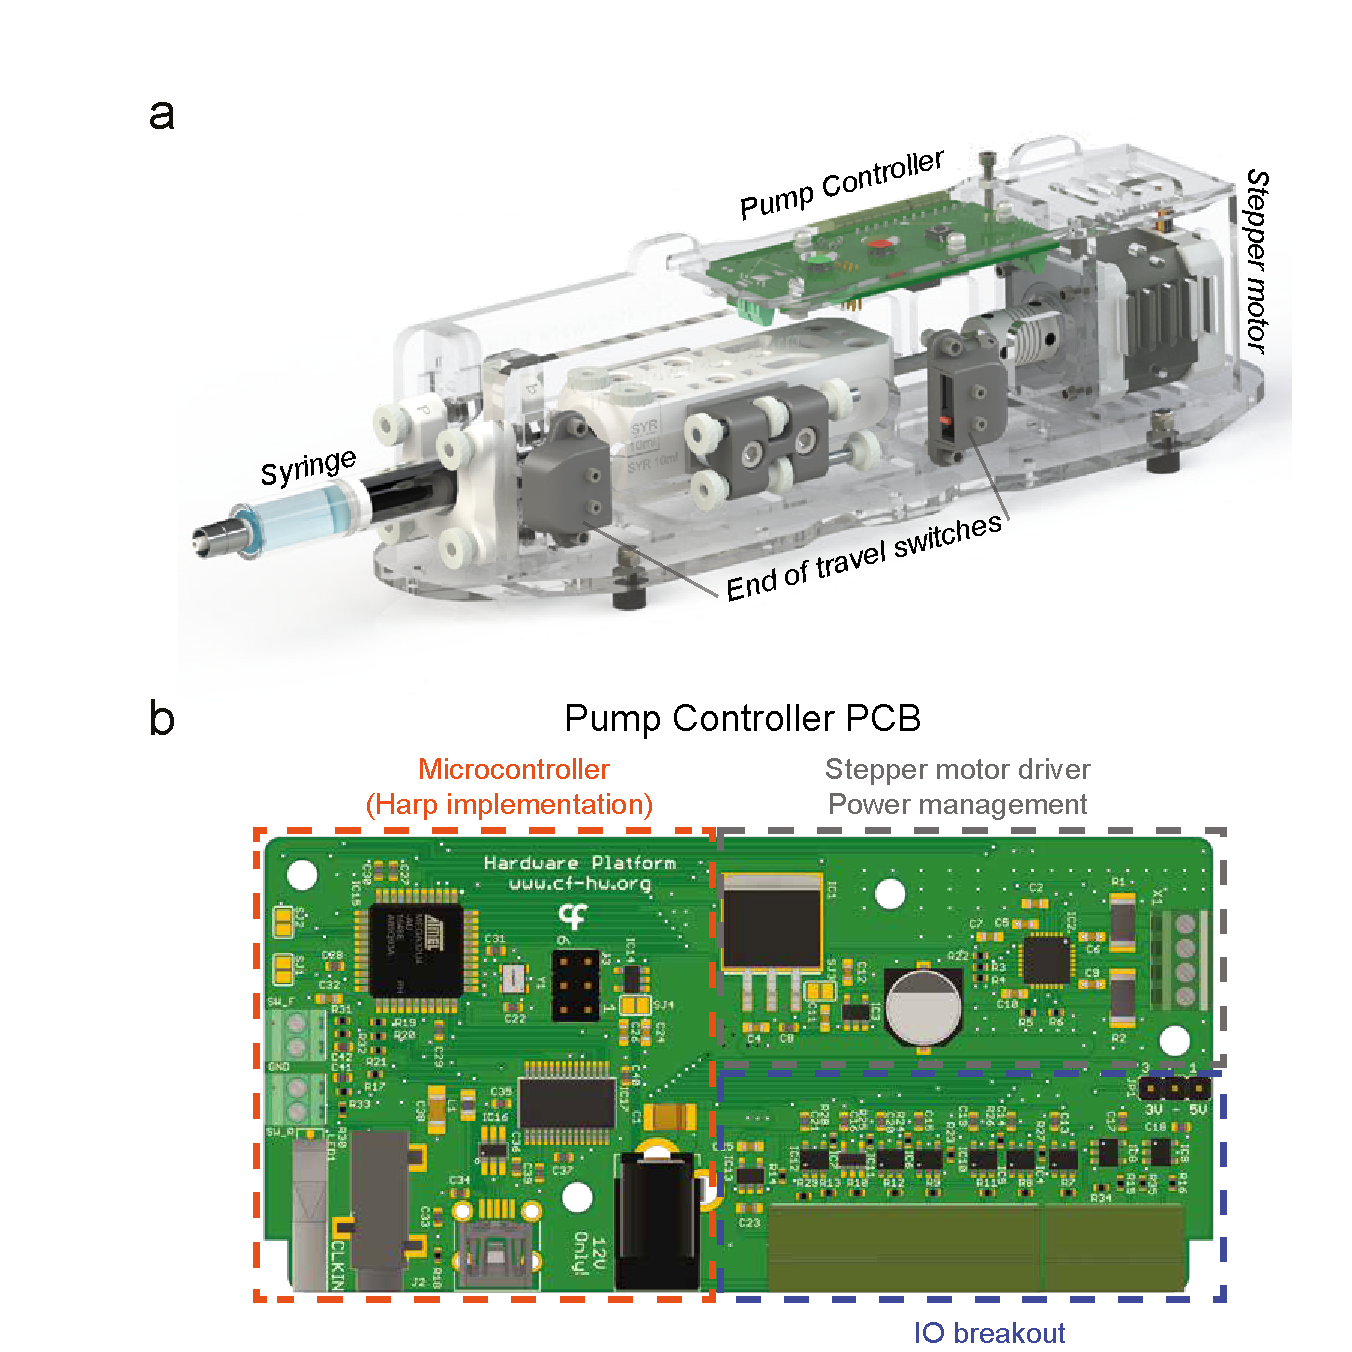
\includegraphics[width=1.0\linewidth]{Figures/Artboard 1.pdf}
	\caption{\textbf{Syringe pump system.}\\
		(\textbf{A}) 3D model of the fully assembled syringe pump system. Controller PCB, Syringe, switches, and stepper motor are highlighted.  \textbf{B}) Diagram of Controller PCB. The three main sections of the board are highlighted: Microcontroller, which implements the Harp protocol; Motor driver and power management, which provide the low-level logic to drive the stepper motor, and the I/O breakout, that affords users with input and output lines which can be used to control and monitor the function of the system, respectively. See \hyperref[s:methods]{Methods} for further details}
	\label{fig:PumpDrawing}
\end{figure*}
